\documentclass[a4j]{jarticle}

\usepackage[dvipdfmx]{graphicx}
\usepackage{url}
\usepackage{listings,jlisting}
\usepackage{ascmac}
\usepackage{amsmath,amssymb}

%ここからソースコードの表示に関する設定
\lstset{
  basicstyle={\ttfamily},
  identifierstyle={\small},
  commentstyle={\smallitshape},
  keywordstyle={\small\bfseries},
  ndkeywordstyle={\small},
  stringstyle={\small\ttfamily},
  frame={tb},
  breaklines=true,
  columns=[l]{fullflexible},
  numbers=left,
  xrightmargin=0zw,
  xleftmargin=3zw,
  numberstyle={\scriptsize},
  stepnumber=1,
  numbersep=1zw,
  lineskip=-0.5ex
}
%ここまでソースコードの表示に関する設定

\title{知能プログラミング演習II 課題3}
\author{グループ07\\
  29114086 飛世裕貴\\
%  {\small (グループレポートの場合は、グループ名および全員の学生番号と氏名が必要)}
}
\date{2019年10月28日}

\begin{document}
\maketitle

\paragraph{提出物} rep3
\paragraph{グループ} グループ07
\paragraph{メンバー}
\begin{tabular}{|c|c|c|}
  \hline\hline
  学籍番号&名前&貢献度\\
  \hline\hline
  29114007&池口弘尚&\\
  \hline
  29114031&大原拓人&\\
  \hline
  29114048&北原太一&\\
  \hline
  29114086&飛世裕貴&\\
  \hline
  29114095&野竹浩二朗&\\
  \hline
\end{tabular}



\section{課題の説明}
\begin{description}
\item[課題3-1] セマンティックネットのプログラムを参考に,グループメンバー全員(およびその周辺人物)についてのセマンティックネットを構築せよ.
個人レポートには自分のみ(とその周辺)に関するセマンティックネットを示し,グループレポートには全員(とその周辺)に関するセマンティックネットを示せ

\item[課題3-2] フレームのプログラムを参考に,自分達の興味分野に関する知識をフレームで表現せよ.その分野の知識を表す上で必須となるスロットが何かを考え,クラスフレームを設計すること.
個人レポートには自分が作ったインスタンスフレームのみ(クラスフレームの設計担当者はクラスフレームも)を示し,グループレポートにはクラスフレームおよび全員分のインスタンスフレームを示せ.
\item[課題3-3] 課題3-1または3-2で作った知識表現を用いた質問応答システムを作成せよ.
なお,ユーザの質問は英語や日本語のような自然言語が望ましいが,難しければ課題2で扱ったような変数を含むパターン (クエリー) でも構わない.

\item[課題3-4]課題3-1または3-2で作った知識表現を図として示すためのユーザインターフェース(GUI) を設計し実装せよ。
\item[課題3-5] DBpedia Japaneseは,Wikipedia日本語版から生成された知識表現から成る巨大な知識ベースである.またWikidataは,誰でも直接編集できる知識ベースである。
上記3-3で作成した質問応答システムを,DBpediaあるいはWikidata中の知識を使って質問に答えられるよう,拡張せよ.

\end{description}

今回、私が担当した課題は課題3-1、3-2、3-3である。

\section{課題3-1}
\begin{screen}
 セマンティックネットのプログラムを参考に,グループメンバー全員(およびその周辺人物)についてのセマンティックネットを構築せよ.
個人レポートには自分のみ(とその周辺)に関するセマンティックネットを示し,グループレポートには全員(とその周辺)に関するセマンティックネットを示せ
\end{screen}

\subsection{手法}
ここで構築したセマンティックネットは下図のようなものである.

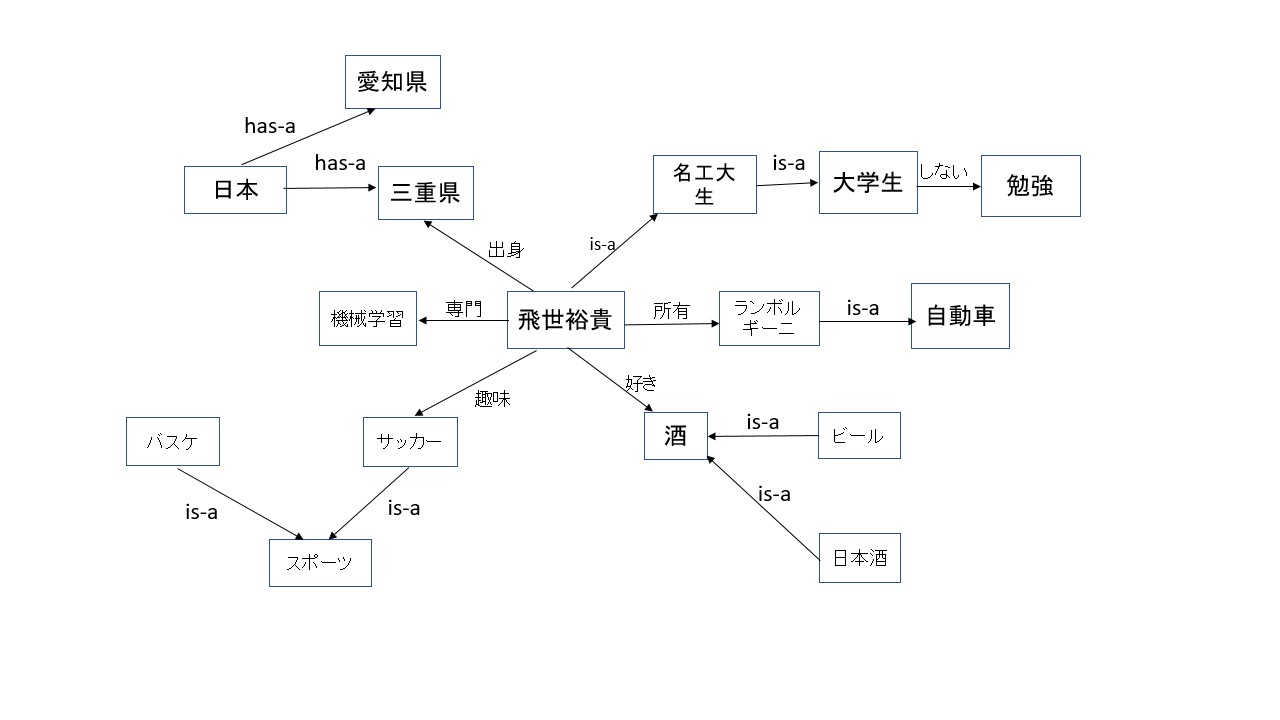
\includegraphics[width=150mm,height=80mm]{Slide2.jpg}

\subsection{実装}
上に示したセマンティックネットをMakeSemanticNet.javaにおいて生成する.セマンティックネットの生成はExample.javaを元に実装した.

\subsection{実行例}
MakeSemanticNet.javaによってセマンティックネットを生成した.その結果を以下に示す.

\begin{screen}
\begin{verbatim}
飛世裕貴  =is-a=>  名工大生
飛世裕貴  =所有=>  ランボルギーニ
飛世裕貴  =好き=>  酒
飛世裕貴  =趣味=>  サッカー
飛世裕貴  =専門=>  機械学習
飛世裕貴  =出身=>  三重県
名工大生  =is-a=>  大学生
( 飛世裕貴  =is-a=>  大学生 )
大学生  =しない=>  勉強
( 名工大生  =しない=>  勉強 )
( 飛世裕貴  =しない=>  勉強 )
ランボルギーニ  =is-a=>  自動車
ビール  =is-a=>  酒
日本酒  =is-a=>  酒
サッカー  =is-a=>  スポーツ
バスケ  =is-a=>  スポーツ
日本  =has-a=>  三重県
日本  =has-a=>  愛知県
\end{verbatim}
\end{screen}

このように図に示したものと同様のセマンティックネットが生成されたことを確認した.
\section{課題3-2}
\begin{screen}
フレームのプログラムを参考に,自分達の興味分野に関する知識をフレームで表現せよ.その分野の知識を表す上で必須となるスロットが何かを考え,クラスフレームを設計すること.
個人レポートには自分が作ったインスタンスフレームのみ(クラスフレームの設計担当者はクラスフレームも)を示し,グループレポートにはクラスフレームおよび全員分のインスタンスフレームを示せ.
\end{screen}

\subsection{手法}
ここでは任天堂の『大乱闘スマッシュブラザーズ』というゲームのキャラクターに関するクラスフレームとインスタンスフレームを構築した.構築したフレームは下図のようなものである.


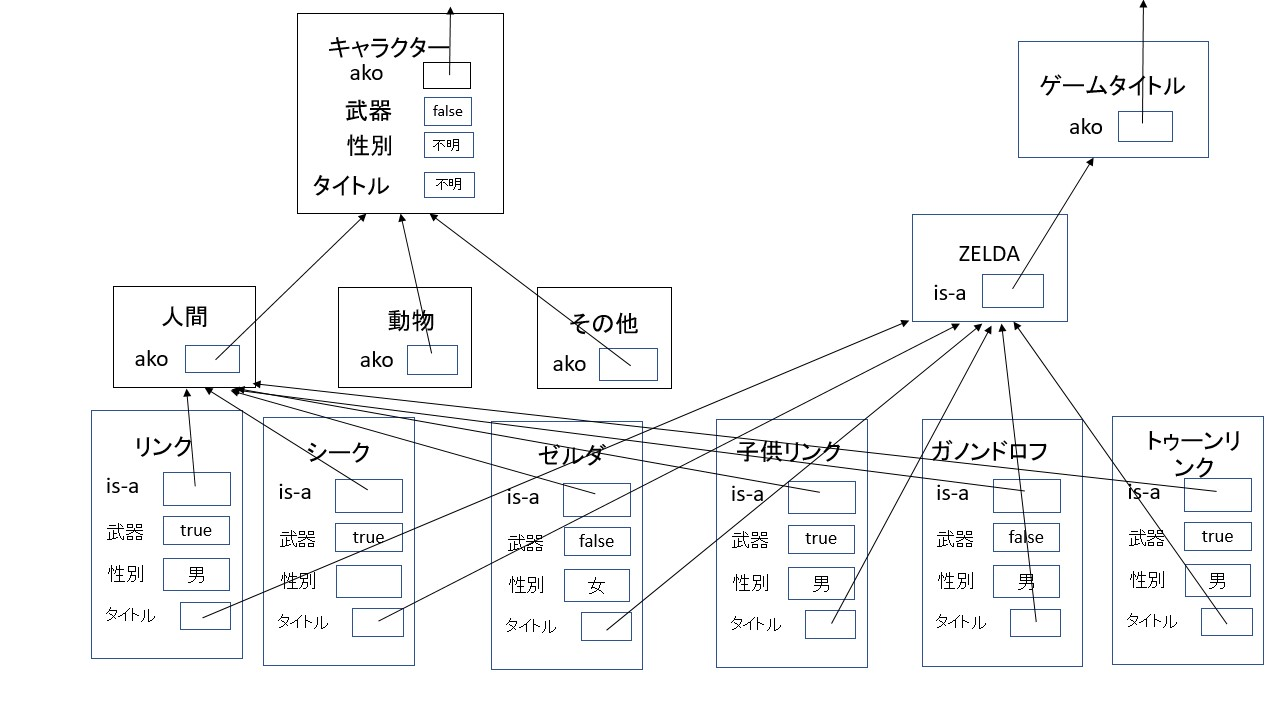
\includegraphics[width=150mm,height=80mm]{Slide1.jpg}

この図において「キャラクター」「人間」「動物」「その他」「ゲームタイトル」フレームをクラスフレーム、それ以外をインスタンスフレームとして構築している。


\subsection{実装}
上に示したフレームをMakeFrame.javaにおいて生成する.フレームの生成はExample.javaを元に実装した.なおフレームの構築
において、キャラクターのスロットにゲームタイトルのインスタンスフレームを格納する必要があったため、生成したフレームを格納しているHashMapからフレームを取り出すgetFrameメソッドをAIFrameSystem.javaに、フレームの名前を取得するgetmNameメソッドをAIFrame.javaに実装した。
\subsection{実行例}
MakeFrame.javaによってフレームを生成した.ここではreadSlotValueメソッドを用いて、生成したフレームにおいて各スロットの値が正しく格納されているかを確認した.その結果の一部を以下に示す.
\\

\begin{screen}
\begin{verbatim}
Frame:リンク
武器:true
性別:男
タイトル:ZELDA
\end{verbatim}
\end{screen}

このように生成したフレームのスロットに正しい値が格納されていることがわかる.また、ここでは『リンク』フレームに関する実行結果のみを示しているが、他のフレームに関しても同様の処理をした結果、図に示したものと同様のフレームが生成されたことを確認した.


\section{課題3-3}
\begin{screen}
課題3-1または3-2で作った知識表現を用いた質問応答システムを作成せよ.
なお,ユーザの質問は英語や日本語のような自然言語が望ましいが,難しければ課題2で扱ったような変数を含むパターン (クエリー) でも構わない.
\end{screen}

\subsection{手法}
ここでは課題2で扱ったような変数を含むパターンによる質問応答システムを課題3-1で生成したセマンティックネットに対して実装した.

\subsection{実装}
質問応答システムはExample.javaを変更することで実装した.以下に変更点を示す.
\\
\begin{lstlisting}[caption=MakeSemanticNetクラスより抜粋]
		Scanner stdin = new Scanner(System.in);
		int size = 0;
		String[] list = new String[3];
		while(size!=3){
			System.out.print("Enter Search Pattern(<Node> <Link> <Node>):");
			String str = stdin.nextLine();
			String[] sentence = str.split("( | )");
			if(sentence.length == 3){
				for(int i = 0;i<3;i++){
					list[i] = sentence[i];
				}
			}
			size = sentence.length;
		}
		ArrayList<Link> query = new ArrayList<Link>();
		query.add(new Link(list[1],list[0],list[2]));
		sn.query(query);
\end{lstlisting}

上記のように質問応答は標準入力から「飛世裕貴 好き ?x」のように「<ノード名> <リンク> <ノード名>」という型のクエリーを取得し、そのクエリーを空白で分割し、queryメソッドを用いてマッチングを行うことで変数?xに該当するものを返すようにした.
\subsection{実行例}
実装した質問応答システムを用いて検索した結果を以下に示す.
\\
\begin{screen}
\begin{verbatim}
Enter Search Pattern:飛世裕貴 ?x ?y
*** Query ***
飛世裕貴  =?x=>  ?y
[{?x=is-a, ?y=名工大生}, {?x=所有, ?y=ランボルギーニ}, {?x=好き, ?y=酒}, {?x=趣味, ?y=サッカー}, {?x=専門, ?y=機械学習}, {?x=出身, ?y=三重県}, {?x=is-a, ?y=大学生}, {?x=しない, ?y=勉強}, {?x=する, ?y=勉強}]

Enter Search Pattern:飛世裕貴 ?x 酒
*** Query ***
飛世裕貴  =?x=>  酒
[{?x=好き}]
\end{verbatim}
\end{screen}


このようにセマンティックネットに対して検索が正常に行われていることを確認した.

\subsection{考察}
今回はセマンティックネットに関して質問応答システムをパターンを用いた方式で実装したが、係り受け解析器CaboChaを用いることでセマンティックネットとフレームのどちらにおいても自然言語を用いた検索が可能になると考えられる.係り受け解析は各形態素の関係を推定するもので、この係り受け解析を行うことで検索語において何の値を要求されているのかを推定することができる.例えば、今回構築したセマンティックネットに対して「飛世裕貴の好きなものは何?」という検索語で要求されているものは「飛世裕貴」というノードから「好き」というリンクで繋がっているノードの値であるというような推定が可能となると考えられる.しかし、このような自然言語による質問応答システムを実装する上で問題となるのは、検索表現の一意性である.先ほどの例のように検索語に現れるノードとリンクの関係がセマンティックネットにおけるグラフの向きと合致している場合はノードを辿っていくことで検索するというように実装が容易であるが、「酒が好きなのは誰?」というようにグラフの向きと検索語におけるノードとリンクの関係が合致しない場合は無向グラフ的にセマンティックネットをとらえるという方法や全ノードに対して「酒」というノードに「好き」というリンクが存在するノードを総当たり探索するなど、セマンティックネットの有用性の喪失や探索時間の増加を引き起こしてしまうと考えられる.\\
このため自然言語による探索を実装したとしてもセマンティックネットやフレームの性質を生かすためには、本質的にパターンマッチングと同等の質問応答システムとなるのではないかと考える.

\section{感想}
\end{document}
